\documentclass[12pt,a4paper,twoside]{report}
% -------------------------------------------------------------------- %
% Pacotes

\usepackage[utf8]{inputenc}
\usepackage[T1]{fontenc}
\usepackage[brazil]{babel}
\usepackage[fixlanguage]{babelbib}
\usepackage[pdftex]{graphicx}      % usamos arquivos pdf/png como figuras
\usepackage{setspace}              % espaçamento flexvel
\usepackage{indentfirst}           % indentação do primeiro parágrafo
\usepackage{makeidx}               % índice remissivo
\usepackage[nottoc]{tocbibind}     % acrescentamos a bibliografia/indice/conteudo no Table of Contents
\usepackage{courier}               % usa o Adobe Courier no lugar de Computer Modern Typewriter
\usepackage{type1cm}               % fontes realmente escaláveis
\usepackage{titletoc}
\usepackage{ucs}
\usepackage[font=small,format=plain,labelfont=bf,up,textfont=it,up]{caption}
\usepackage[usenames,svgnames,dvipsnames]{xcolor}
\usepackage[a4paper,top=2.54cm,bottom=2.0cm,left=2.0cm,right=2.54cm]{geometry} % margens
\usepackage{amsmath} 

\usepackage[pdftex,plainpages=false,pdfpagelabels,pagebackref,colorlinks=true,citecolor=DarkGreen,
linkcolor=NavyBlue,urlcolor=DarkRed,filecolor=green,bookmarksopen=true]{hyperref} % links coloridos
\usepackage[all]{hypcap}                % soluciona o problema com o hyperref e capítulos
\usepackage[square,sort,nonamebreak,comma]{natbib}  % citação bibliográfica alpha
\fontsize{60}{62}\usefont{OT1}{cmr}{m}{n}{\selectfont}
\usepackage{upquote}                    % formata apóstrofes '
\usepackage{textcomp}

% Para formatar corretamente as URLs
\usepackage{url}
% -------------------------------------------------------------------- %
% Cabeçalhos similares ao TAOCP de Donald E. Knuth
\usepackage{fancyhdr}
\pagestyle{fancy}
\fancyhf{}
\renewcommand{\chaptermark}[1]{\markboth{\MakeUppercase{#1}}{}}
\renewcommand{\sectionmark}[1]{\markright{\MakeUppercase{#1}}{}}
\renewcommand{\headrulewidth}{0pt}

% -------------------------------------------------------------------- %
\graphicspath{{./imagens/}}        % caminho das figuras
\frenchspacing                     % arruma o espaço: id est (i.e.) e exempli gratia (e.g.)
\urlstyle{same}                    % URL com o mesmo estilo do texto e no mono-spaced
\makeindex                         % para o índice remissivo
\raggedbottom                      % para no permitir espaços extras no texto
\fontsize{60}{62}\usefont{OT1}{cmr}{m}{n}{\selectfont}
\cleardoublepage
\normalsize

% -------------------------------------------------------------------- %
% Cores para formatação de código
\usepackage{color}
\definecolor{vermelho}{rgb}{0.6,0,0} % para strings
\definecolor{verde}{rgb}{0.25,0.5,0.35} % para comentários
\definecolor{roxo}{rgb}{0.5,0,0.35} % para palavras-chaves
\definecolor{azul}{rgb}{0.25,0.35,0.75} % para strings
\definecolor{cinza-claro}{gray}{0.95}
% -------------------------------------------------------------------- %
% Opções de listagem usados para o código fonte
% Ref: http://en.wikibooks.org/wiki/LaTeX/Packages/Listings



\usepackage{listings}           % para formatar código-fonte (ex. em Java)


\lstset{ %
language=[Objective]Caml,  % seleciona a linguagem do código (aqui em lstlang0.sty
basicstyle=\footnotesize\ttfamily, % o tamanho da fonte usado no código
commentstyle=\color{verde}\bfseries,  % formatação de comentários
stringstyle=\color{azul},    % formatação de strings
upquote=true,
numbers=left,                   % onde colocar os números de linha
numberstyle=\tiny,  % o tamanho da fonte usada para a numeração das linhas
stepnumber=1,                   % o intervalo entre dois números de linhas. Se for 1, numera cada uma.
numbersep=5pt,                  % how far the line-numbers are from the code
showspaces=false,               % show spaces adding particular underscores
showstringspaces=false,         % underline spaces within strings
showtabs=false,                 % show tabs within strings adding particular underscores
keywordstyle=\color{roxo}\bfseries,
keywordstyle=[1]\color{roxo}\bfseries,
keywordstyle=[2]\color{verde}\bfseries,
%        keywordstyle=[3]\textbf,    %
%        keywordstyle=[4]\textbf,   \sqrt{\sqrt{}} %
frame=b,                   % adds a frame around the code
framerule=0.6pt,
tabsize=2,                      % sets default tabsize to 2 spaces
captionpos=t,                   % sets the caption-position to top
breaklines=true,                % sets automatic line breaking
breakatwhitespace=false,        % sets if automatic breaks should only happen at whitespace
escapeinside={\%*}{*)},         % if you want to add a comment within your code
backgroundcolor=\color[rgb]{1.0,1.0,1.0}, % choose the background color.
rulecolor=\color[rgb]{0.8,0.8,0.8},
extendedchars=true,
xleftmargin=10pt,
xrightmargin=10pt,
framexleftmargin=10pt,
framexrightmargin=10pt,
literate={â}{{\^{a}}}1  % para formatar corretamente os acentos do Português ao usar utf8
    {ê}{{\^{e}}}1
    {ô}{{\^{o}}}1  
    {Â}{{\^{A}}}1
    {Ê}{{\^{E}}}1
    {Ô}{{\^{O}}}1
    {á}{{\'{a}}}1
    {é}{{\'{e}}}1
    {í}{{\'{i}}}1
    {ó}{{\'{o}}}1
    {ú}{{\'{u}}}1
    {Á}{{\'{A}}}1
    {É}{{\'{E}}}1
    {Í}{{\'{I}}}1
    {Ó}{{\'{O}}}1
    {Ú}{{\'{U}}}1
    {à}{{\`{a}}}1
    {À}{{\`{A}}}1
    {ã}{{\~{a}}}1
    {õ}{{\~{o}}}1
    {Ã}{{\~{A}}}1
    {Õ}{{\~{O}}}1
    {ç}{{\c{c}}}1
    {Ç}{{\c{C}}}1
    {ü}{{\"u}}1
    {Ü}{{\"U}}1
}

\renewcommand{\lstlistingname}{Listagem}
\renewcommand{\lstlistlistingname}{Lista de Listagens}

% Definição de novos estilos
\lstdefinestyle{Bash}
    {language=bash,frame=single,numbers=none,basicstyle=\footnotesize\ttfamily,
     morekeywords={cp,mkdir,sudo,tar}}

% Definição de novos ambientes
\lstnewenvironment{terminal}
  {\lstset{style=Bash}}
  {}

\lstnewenvironment{ocaml}
  {\lstset{basicstyle=\scriptsize\ttfamily,
           frame=single,
           frameround=tttt,
           framerule=2pt,
           numbers=none,
           rulecolor=\color{Salmon}}}
  {}

\lstnewenvironment{xml}
   {\lstset{language=XML,frame=single,numbers=none}}
   {}

\lstnewenvironment{interprete}
  {\lstset{frame=single,
            frameround=tttt,
            numbers=none,
            basicstyle=\ttfamily,
            framerule=2pt,
            rulecolor=\color{CadetBlue}}}
  {}
% Formata o caption da listagem
% \DeclareCaptionFont{blue}{\color{blue}} 

% \captionsetup[lstlisting]{singlelinecheck=false, labelfont={blue}, textfont={blue}}
\usepackage{caption}
\DeclareCaptionFont{white}{\color{white}}
\DeclareCaptionFormat{listing}{\colorbox[cmyk]{0.43, 0.35, 0.35,0.01}{\parbox{\textwidth}{\hspace{15pt}#1#2#3}}}
\captionsetup[lstlisting]{format=listing,labelfont=white,textfont=white, singlelinecheck=false, margin=0pt, font={bf,footnotesize}}

\newcommand{\ListingsPath}{./codigos}
% Inclui o nome do arquivo como Caption 
\newcommand{\filelisting}[2][]{%
    \lstinputlisting[caption={\texttt{\detokenize{#2}}},#1]{\ListingsPath/#2}%
}

% ---------------------------------------------------------------------------- %

% ---------------------------------------------------------------------------- %

\title{Construção de um compilador de MiniJava para Dalvik usando Objective Caml}
\date{}
\author{Fulano \\
\texttt{\small \url{fulano@gmail.com}}\\
Ciclano \\
\texttt{\small \url{ciclano@gmail.com}}\\
Beltrano \\
\texttt{\small \url{beltrano@gmail.com}}\\
\vspace{1cm} \\
Faculdade de Computação \\
Universidade Federal de Uberlândia
}
\date{\today}

%\includeonly{cap-clojure,magical,short}
\begin{document}
  \maketitle
% -------------------------------------------------------------------- %
% Listas de figuras, tabelas e códigos criadas automaticamente
\listoffigures            
\listoftables            
\lstlistoflistings
% -------------------------------------------------------------------- %

% -------------------------------------------------------------------- %
% Sumário
\tableofcontents    

% Capítulos do trabalho

% cabeçalho para as páginas de todos os capítulos
\fancyhead[RE,LO]{\thesection}

%\singlespacing              % espaçamento simples
\setlength{\parskip}{0.15in} % espaçamento entre paragráfos

\chapter{Introdução}
Este documento foi escrito para auxiliar na confecção do relatório da
disciplina. É necessário olhar os fontes deste documento em \LaTeX\ para
compreender algumas coisas.

\section{Linha de comando}
Para dar instruções sobre linha de comando use um ambiente que preparei
(veja o preâmbulo desse documento para aprender como criar seu próprio
ambiente):

\begin{verbatim}
\begin{terminal}
> sudo apt-get install tree
\end{terminal}
\end{verbatim}

Um programa bastante útil é o \verb|tree| que lista o conteúdo de um
diretório e de seus subdiretórios em forma de árvore. Para instalá-lo no
Ubuntu, use:

\begin{terminal}
> sudo apt-get install tree
\end{terminal}

A seguir é mostrado o uso:
\begin{terminal}
> tree --charset=ASCII
.
|-- codigos
|   |-- exemplo1.ml
|   `-- MiniJava
|       |-- fact.mj
|       `-- prog1.mj
|-- compiladores.aux
|-- compiladores.idx
|-- compiladores.lof
|-- compiladores.log
|-- compiladores.lol
|-- compiladores.lot
|-- compiladores.out
|-- compiladores.pdf
|-- compiladores.tex
|-- compiladores.toc
`-- relatorio.tex

2 directories, 14 files
\end{terminal}

\section{Códigos de programas}
Para introduzir a listagem do código no documento existem pelo menos duas
formas básicas, ambas usando o pacote \verb|listings|:
\begin{enumerate}
\item Diretamente do documento \LaTeX\ usando por exemplo
\begin{verbatim}
\begin{ocaml}
type binop =
    Plus
  | Minus
  | Times
  | Div
  | Mod
  | Le
  | Leq
  | Ge
  | Geq
  | Eq
  | Neq
  | And
  | Or
\end{ocaml}
\end{verbatim}
cujo resultado é
\begin{ocaml}
type binop =
    Plus
  | Minus
  | Times
  | Div
  | Mod
  | Le
  | Leq
  | Ge
  | Geq
  | Eq
  | Neq
  | And
  | Or
\end{ocaml}  
\item Lendo o código diretamente do arquivo:
\begin{verbatim}
\lstinputlisting[caption={exemplo1.ml}]{codigos/exemplo1.ml}
\end{verbatim}
cujo resultado é mostrado na listagem~\ref{arq:exemplo1}.

\lstinputlisting[caption={exemplo1.ml \label{arq:exemplo1}}]{codigos/exemplo1.ml}
\end{enumerate}

\chapter{Imagens}

Se desejar incluir imagens você poderá usar o comando a seguir:

\begin{verbatim}
\begin{figure}[!ht]
\centering
\caption{Página de entrada do site 
     \url{http://studiosum.com.br/CC1/index.php} \label{fig:1}}
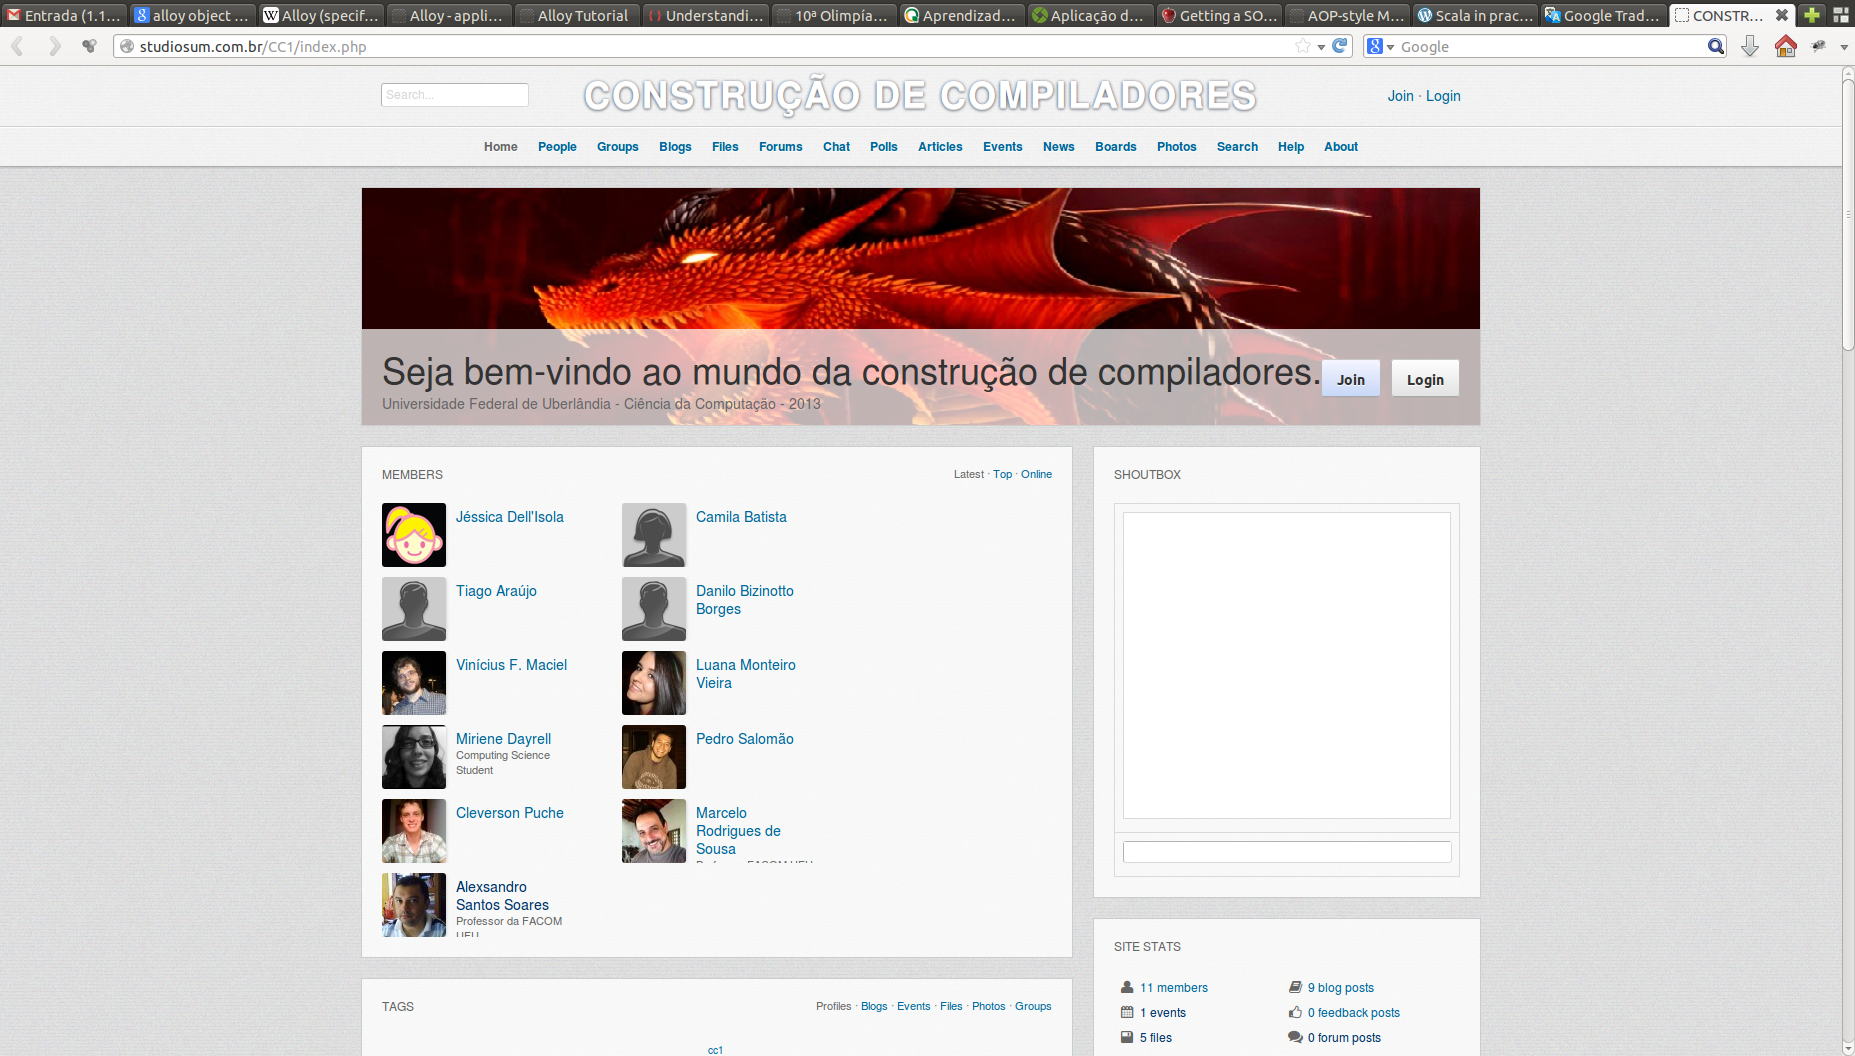
\includegraphics[scale=0.27]{imagens/fig1.png}
\end{figure}
\end{verbatim}

O comando anterior gerará a imagem a seguir, dado que o arquivo \texttt{fig1.png} esteja no subdiretório \texttt{imagens}.
\begin{figure}[!h]
\centering
\caption{Página de entrada do site \url{http://studiosum.com.br/CC1/index.php} \label{fig:1}}
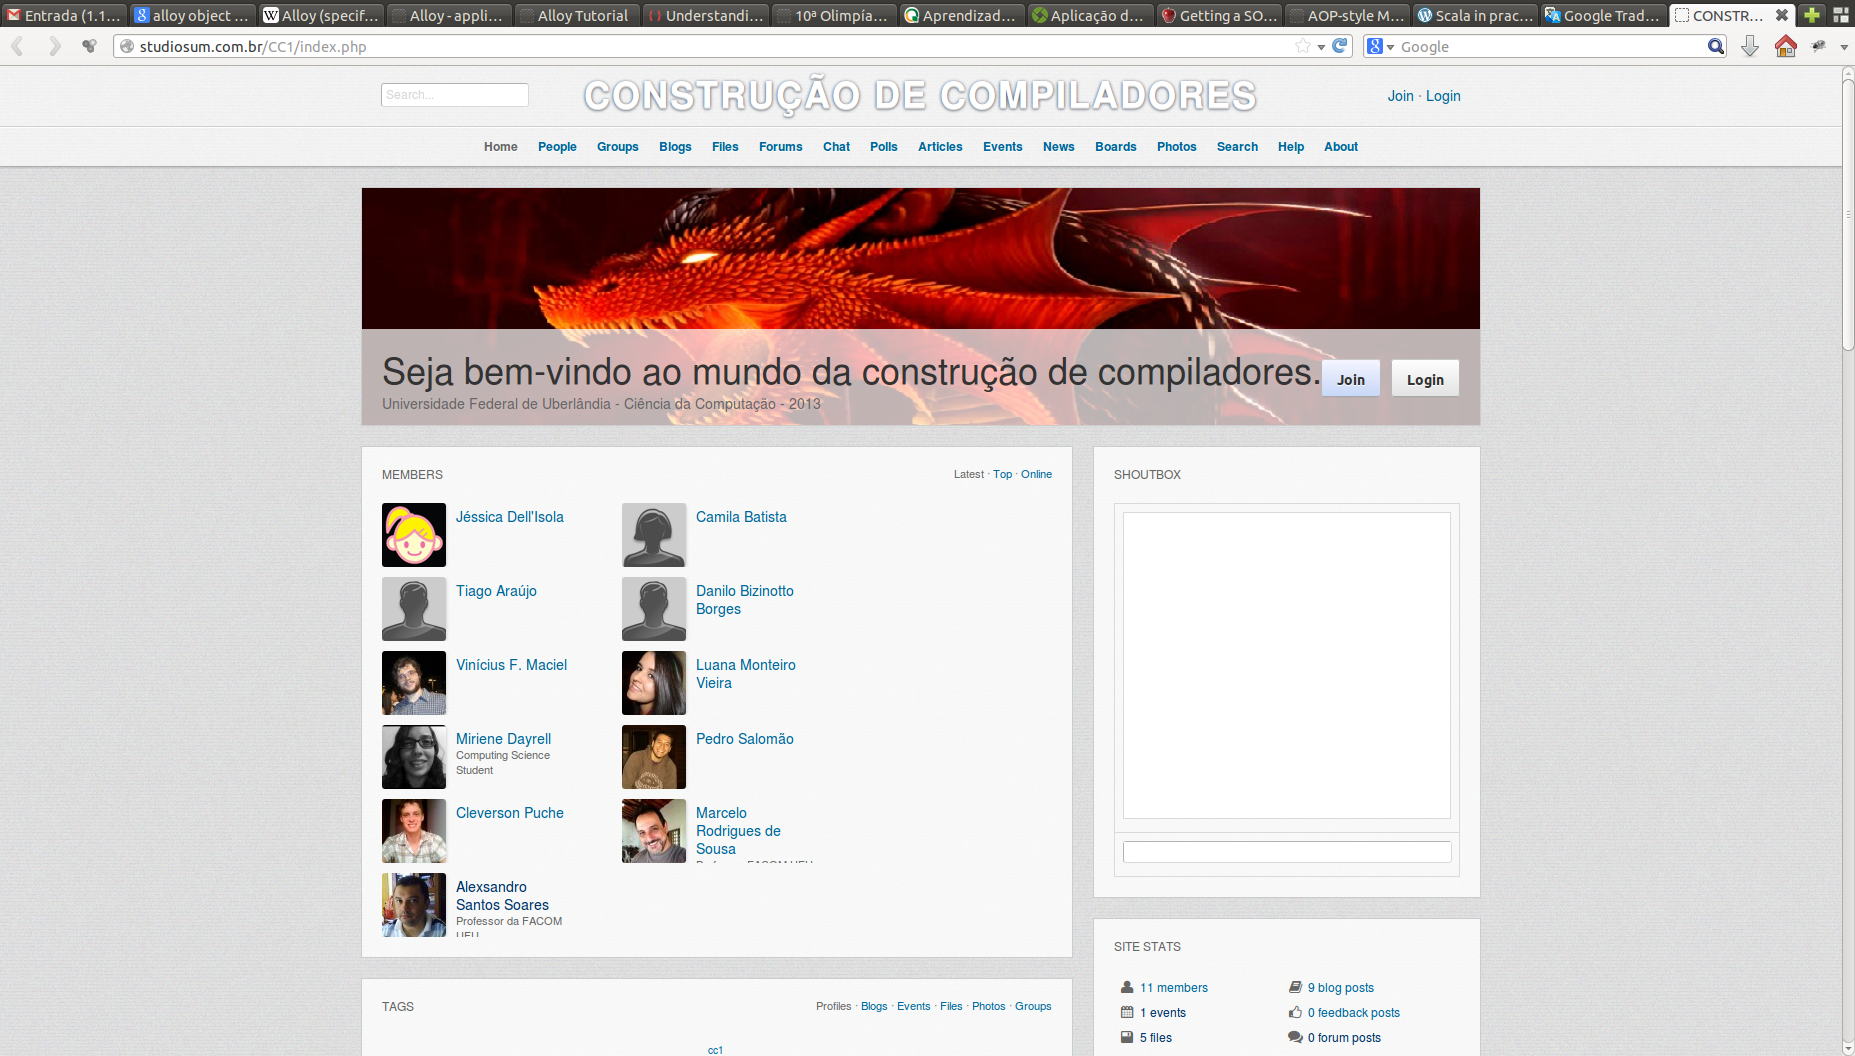
\includegraphics[scale=0.25]{imagens/fig1.png}
\end{figure}

Note que a Figura~\ref{fig:1} pode ser referenciada em qualquer parte do documento.  Você também pode incluir diretamente outros formatos de imagens tais como o \texttt{jpg}.


\clearpage
\addcontentsline{toc}{part}{Apêndice}
\appendix

\chapter{Exemplos de programas escritos em MiniJava \label{ap:Testes}}
\section{prog1.mj}
\lstinputlisting[label={arq:prog1.mj}, language=Java,
caption={prog1.mj}]{codigos/MiniJava/prog1.mj}

\section{fact.mj}

\lstinputlisting[label={arq:fact.mj}, language=Java,
caption={prog1.mj}]{codigos/MiniJava/fact.mj}


\end{document} 
